% -----------------------------*- LaTeX -*------------------------------
\documentclass[UTF8]{report}
% ------------------------------------------------------------------------
% Packages
% ------------------------------------------------------------------------
\usepackage{adjustbox}
\usepackage{algorithm,algorithmicx}
\usepackage[noend]{algpseudocode}
\usepackage{amsmath,amsfonts,amssymb,bm,amsthm}%数学宏包、数学字体、数学符号、支持 \mathscr{} 字体、支持粗斜体 \bm{}、数学定理
\usepackage{bigstrut,multirow,rotating}%Excel表格自动导入latex
\usepackage{booktabs}
\usepackage{breqn}
\usepackage{caption}
\usepackage{color}%支持颜色改变
\usepackage{ctex}
\usepackage{enumitem}%自定义列表环境
\usepackage{esint}%支持多种积分算子
\usepackage{extarrows}%任意长度的箭头
\usepackage{fancyhdr}
\usepackage{fontsize}
\usepackage{fontspec}
\usepackage[body={7in, 9in},left=1in,right=1in]{geometry}
\usepackage{graphicx}%支持 \includegraphics{} 插图
\usepackage{mathrsfs}
\usepackage{mathtools}%数学宏包的重要补充
\usepackage[framemethod=TikZ]{mdframed}
\usepackage{nicefrac}
\usepackage{scribe}
\usepackage{subfigure}%插入子图
\usepackage{tikz,xcolor}%画图、画 Feynman 图
\usepackage{upgreek}%数学环境的直立希腊字母
% ------------------------------------------------------------------------
% Macros
% ------------------------------------------------------------------------
%~~~~~~~~~~~~~~~
% Utility latin
%~~~~~~~~~~~~~~~
\newcommand{\ie}{\textit{i.e.}}
\newcommand{\eg}{\textit{e.g.}}
%~~~~~~~~~~~~~~~
% Environment shortcuts
%~~~~~~~~~~~~~~~
\newcommand{\balign}[1]{\ealign{\begin{align}#1\end{align}}}
\newcommand{\baligns}[1]{\ealigns{\begin{align*}#1\end{align*}}}
\newcommand{\bitemize}[1]{\eitemize{\begin{itemize}#1\end{itemize}}}
\newcommand{\benumerate}[1]{\eenumerate{\begin{enumerate}#1\end{enumerate}}}
%~~~~~~~~~~~~~~~
% Text with quads around it
%~~~~~~~~~~~~~~~
\newcommand{\qtext}[1]{\quad\text{#1}\quad}
%~~~~~~~~~~~~~~~
% Shorthand for math formatting
%~~~~~~~~~~~~~~~
\newcommand{\mbb}[1]{\mathbb{#1}}
\newcommand{\mbi}[1]{\boldsymbol{#1}} % Bold and italic (math bold italic)
\newcommand{\mbf}[1]{\mathbf{#1}}
\newcommand{\mc}[1]{\mathcal{#1}}
\newcommand{\mrm}[1]{\mathrm{#1}}
\newcommand{\tbf}[1]{\textbf{#1}}
\newcommand{\tsc}[1]{\textsc{#1}}
%\def\<{{\langle}}
%\def\>{{\rangle}}
\newcommand{\sT}{\sf T}
\newcommand{\grad}{\nabla}
\newcommand{\Proj}{\Pi}
%~~~~~~~~~~~~~~~
% Common sets 定义数集符号
%~~~~~~~~~~~~~~~
\newcommand{\R}{\mathbb{R}}
\newcommand{\Z}{\mathbb{Z}}
\newcommand{\Q}{\mathbb{Q}}
\newcommand{\N}{\mathbb{N}}
\newcommand{\C}{\mathbb{C}}
\newcommand{\reals}{\mathbb{R}} % Real number symbol
\newcommand{\integers}{\mathbb{Z}} % Integer symbol
\newcommand{\rationals}{\mathbb{Q}} % Rational numbers
\newcommand{\naturals}{\mathbb{N}} % Natural numbers
\newcommand{\complex}{\mathbb{C}} % Complex numbers
%~~~~~~~~~~~~~~~
% Common functions
%~~~~~~~~~~~~~~~
\renewcommand{\exp}[1]{\operatorname{exp}\left(#1\right)} % Exponential
\newcommand{\indic}[1]{\mbb{I}\left(#1\right)} % Indicator function
\newcommand{\indicsub}[2]{\mbb{I}_{#2}\left(#1\right)} % Indicator function
\newcommand{\argmax}{\mathop\mathrm{arg\, max}} % Defining math symbols
\newcommand{\argmin}{\mathop\mathrm{arg\, min}}
\renewcommand{\arccos}{\mathop\mathrm{arccos}}
\newcommand{\dom}{\mathop\mathrm{dom}} % Domain
\newcommand{\range}{\mathop\mathrm{range}} % Range
\newcommand{\diag}{\mathop\mathrm{diag}}
\newcommand{\tr}{\mathop\mathrm{tr}}
\newcommand{\abs}{\mathop\mathrm{abs}}
\newcommand{\card}{\mathop\mathrm{card}}
\newcommand{\sign}{\mathop\mathrm{sign}}
\newcommand{\prox}{\mathrm{prox}} % prox
\newcommand{\rank}[1]{\mathrm{rank}(#1)}
\newcommand{\supp}[1]{\mathrm{supp}(#1)}
\newcommand{\norm}[1]{\lVert#1\rVert}
%~~~~~~~~~~~~~~~
% Common probability symbols
%~~~~~~~~~~~~~~~
\newcommand{\family}{\mathcal{P}} % probability family / statistical model
\newcommand{\iid}{\stackrel{\mathrm{iid}}{\sim}}
\newcommand{\ind}{\stackrel{\mathrm{ind}}{\sim}}
\newcommand{\E}{\mathbb{E}} % Expectation symbol
\newcommand{\Earg}[1]{\E\left[#1\right]}
\newcommand{\Esubarg}[2]{\E_{#1}\left[#2\right]}
\renewcommand{\P}{\mathbb{P}} % Probability symbol
\newcommand{\Parg}[1]{\P\left(#1\right)}
\newcommand{\Psubarg}[2]{\P_{#1}\left[#2\right]}
%\newcommand{\Cov}{\mrm{Cov}} % Covariance symbol
%\newcommand{\Covarg}[1]{\Cov\left[#1\right]}
%\newcommand{\Covsubarg}[2]{\Cov_{#1}\left[#2\right]}
%\newcommand{\model}{\mathcal{P}} % probability family / statistical model
%~~~~~~~~~~~~~~~
% Distributions
%~~~~~~~~~~~~~~~
%\newcommand{\Gsn}{\mathcal{N}}
%\newcommand{\Ber}{\textnormal{Ber}}
%\newcommand{\Bin}{\textnormal{Bin}}
%\newcommand{\Unif}{\textnormal{Unif}}
%\newcommand{\Mult}{\textnormal{Mult}}
%\newcommand{\NegMult}{\textnormal{NegMult}}
%\newcommand{\Dir}{\textnormal{Dir}}
%\newcommand{\Bet}{\textnormal{Beta}}
%\newcommand{\Gam}{\textnormal{Gamma}}
%\newcommand{\Poi}{\textnormal{Poi}}
%\newcommand{\HypGeo}{\textnormal{HypGeo}}
%\newcommand{\GEM}{\textnormal{GEM}}
%\newcommand{\BP}{\textnormal{BP}}
%\newcommand{\DP}{\textnormal{DP}}
%\newcommand{\BeP}{\textnormal{BeP}}
%\newcommand{\Exp}{\textnormal{Exp}}
%~~~~~~~~~~~~~~~
% Theorem-like environments
%~~~~~~~~~~~~~~~
%\theoremstyle{definition}
%\newtheorem{definition}{Definition}
%\newtheorem{example}{Example}
%\newtheorem{problem}{Problem}
%\newtheorem{lemma}{Lemma}
%~~~~~~~~~~~~~~~
% 组合数学的模板和作业里用到的一些宏包和自定义命令
%~~~~~~~~~~~~~~~
\renewcommand{\emph}[1]{\begin{kaishu}#1\end{kaishu}}
\newcommand{\falfac}[1]{^{\underline{#1}}}
\newcommand{\binomfrac}[2]{\frac{#1^{\underline{#2}}}{#2!}}
\newcommand{\ceil}[1]{\left\lceil #1 \right\rceil}
\newcommand{\floor}[1]{\left\lfloor #1 \right\rfloor}
\newcommand{\suminfty}[2]{\sum_{#1=#2}^{\infty}}
\newcommand{\suminftyk}[0]{\sum_{k=0}^{\infty}}
\newcommand{\sumint}[3]{\sum_{#1=#2}^{#3}}
\newcommand{\sumintk}[2]{\sum_{k=#1}^{#2}}
\newcommand{\suminti}[2]{\sum_{i=#1}^{#2}}
%~~~~~~~~~~~~~~~
% 定义新命令
%~~~~~~~~~~~~~~~
\newcommand{\unit}[1]{\,\mathrm{#1}}%用来输出物理量
\newcommand{\dif}{\mathop{}\!\mathrm{d}}%微分算子 d
\newcommand{\pdif}{\mathop{}\!\partial}%偏微分算子
\newcommand{\cdif}{\mathop{}\!\nabla}%协变导数、nabla 算子
\newcommand{\laplace}{\mathop{}\!\Delta}%laplace 算子
\newcommand{\deriv}[3]{\frac{\partial^{#1} #2}{\partial {#3^{#1}}}}
\newcommand{\me}[1]{\mathrm{e}^{#1}}%e 指数
\newcommand{\mi}{\mathrm{i}}%虚数单位
%\newcommand{\mc}{\mathrm{c}}%光速 定义与mathcal冲突
\newcommand{\red}[1]{\textcolor{red}{#1}}
\newcommand{\blue}[1]{\textcolor{blue}{#1}}
%\newcommand{\Rome}[1]{\setcounter{rome}{#1}\Roman{rome}}
%~~~~~~~~~~~~~~~
% 一些数学的环境设置
%~~~~~~~~~~~~~~~
%\newcounter{counter_exm}\setcounter{counter_exm}{1}
%\newcounter{counter_prb}\setcounter{counter_prb}{1}
%\newcounter{counter_thm}\setcounter{counter_thm}{1}
%\newcounter{counter_lma}\setcounter{counter_lma}{1}
%\newcounter{counter_dft}\setcounter{counter_dft}{1}
%\newcounter{counter_clm}\setcounter{counter_clm}{1}
%\newcounter{counter_cly}\setcounter{counter_cly}{1}
%\newtheorem{theorem}{{\hskip 1.7em \bf 定理}}
%\newtheorem{lemma}[theorem]{\hskip 1.7em 引理}
%\newtheorem{proposition}[theorem]{Proposition}
%\newtheorem{claim}[theorem]{\hskip 1.7em 命题}
%\newtheorem{corollary}[theorem]{\hskip 1.7em 推论}
%\newtheorem{definition}[theorem]{\hskip 1.7em 定义}
\newcommand{\problem}[1]{{\setlength{\parskip}{10pt}\noindent \bf{#1}}}
\newenvironment{solution}{{\noindent\hskip 2em \bf 解 \quad}}{}
\renewenvironment{proof}{{\setlength{\parskip}{7pt}\noindent\hskip 2em \bf 证明 \quad}}{\hfill$\qed$\par}
%\newenvironment{example}{{\noindent\hskip 2em \bf 例 \arabic{counter_exm}\quad}}{\addtocounter{counter_exm}{1}\par}
%\newenvironment{concept}[1]{{\bf #1\quad} \begin{kaishu}} {\end{kaishu}\par}

% ----------------------------------------------------------------------
% Header information
% ------------------------------------------------------------------------

\begin{document}

\course{B0911006Y-01} 			%optional
\coursetitle{Computer Organization and Design}	%optional
\semester{2023 Spring}		%optional
\lecturer{Ke Zhang}	%optional
\scribe{吉骏雄}		%required
\lecturenumber{1}			%required (must be a number)
\lecturedate{March 6}	%required (omit year)

\maketitle

% ----------------------------------------------------------------------
% Body of the document
% ------------------------------------------------------------------------


%《计算机组成原理》(唐朔飞版)课后习题1.7, 1.9, 1.10, 1.11, 9.8

\problem{1.7} 解释概念:主机、CPU、主存、存储单元、存储元件、存储基元、存储元、存储字、存储字长、存储容量、机器字长、指令字长。

\begin{solution}
    
    主机:CPU和主存的合称。
    
    CPU:运算器和控制器的合称,中文名为中央处理器。运算器用来完成运算、暂存运算结果,控制器用来控制程序执行、数据传输、处理运算结果。
    
    主存:主存储器,又称内存,是存储器子系统中的一类,用来存放程序和数据,可以直接与CPU交换信息,与辅存相区分。主存包含若干存储单元。
    
    存储单元:包含若干存储元件,可用于存储一串二进制代码。
    
    存储元件:能寄存一位二进制代码“0”或“1”。
    
    存储基元:同“存储元件”。
    
    存储元:同“存储元件”。
    
    存储字:称一个存储单元可存储的一串二进制代码为一个存储字。
    
    存储字长:一个存储单元可存储的这串二进制代码的长度称为存储字长。
    
    存储容量:由主存容量和辅存容量组成。主存容量指住村中存放二进制代码的总位数,即存储单元个数×存储字长;辅存容量则通常用字节数表示。
    
    机器字长:CPU一次能处理数据的位数。
    
    指令字长:一条指令的二进制代码长度。

\end{solution}

\problem{1.9} 画出主机框图,分别以存数指令“STA M”和加法指令“ADD M”(M均为主存地址)为例,在图中按序标出完成该指令(包括取指阶段)的信息流程。假设主存容量为256M×32位,在指令字长、存储字长、机器字长相等的条件下,指出图中各寄存器的位数。

\begin{solution}
    如图\ref{fig0109}.

    \begin{figure}[htbp]
        \centering
        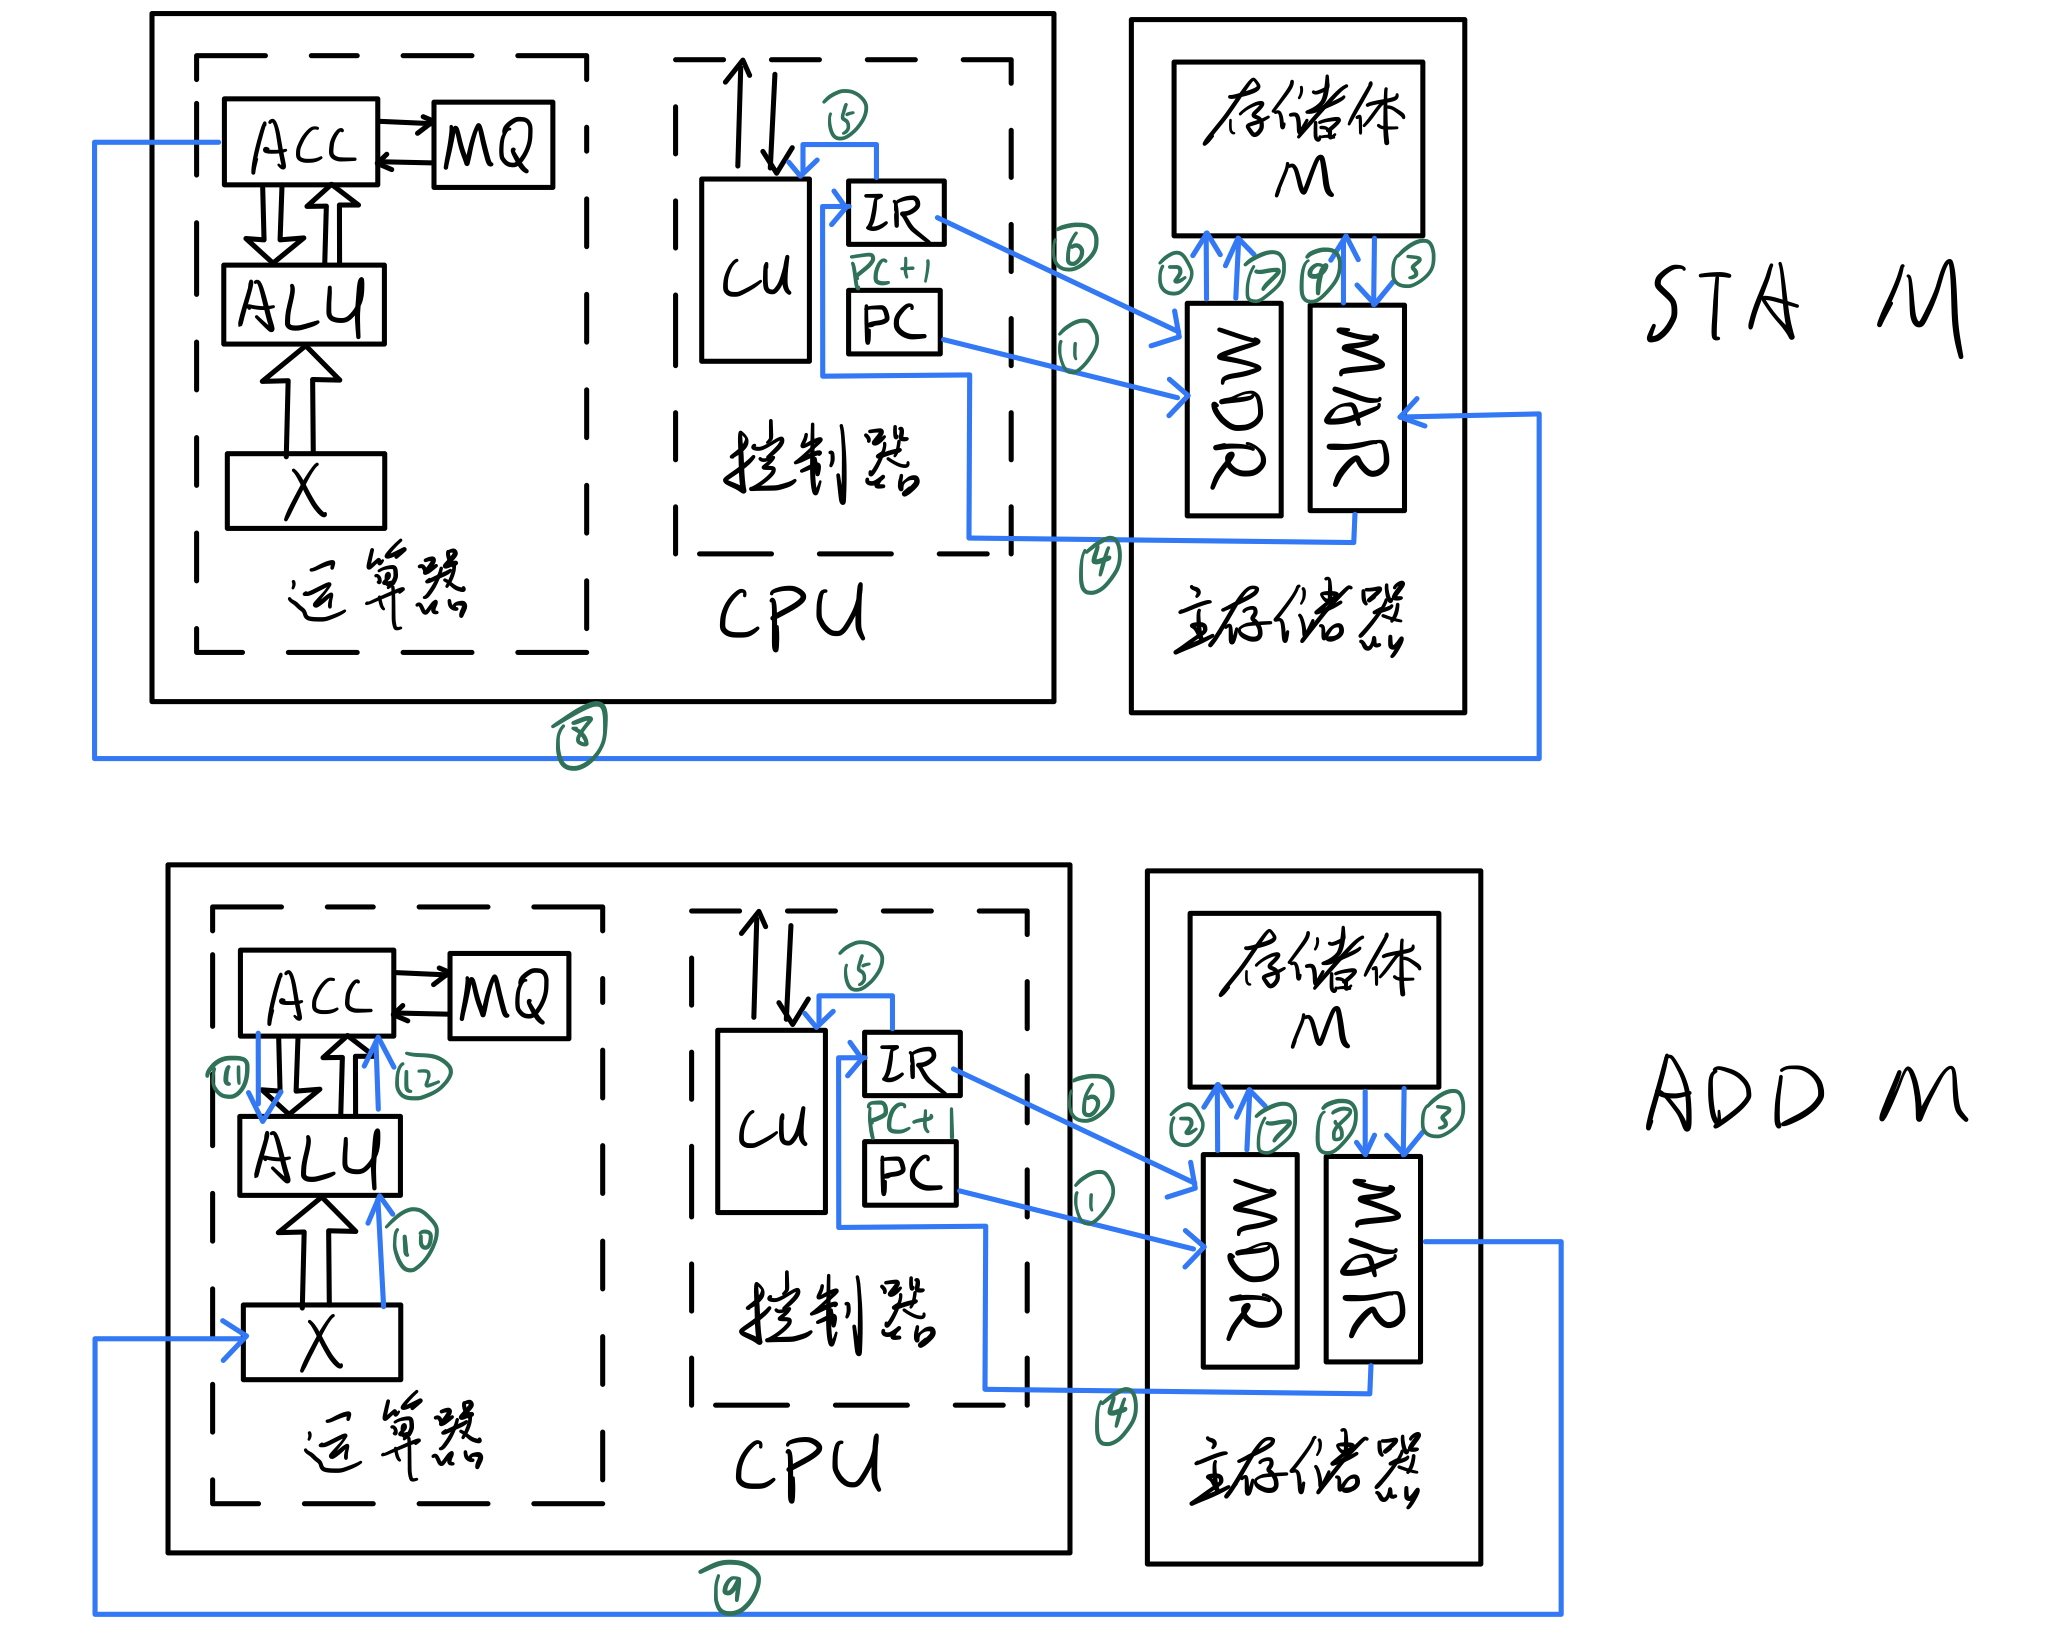
\includegraphics[width=10cm]{fig/1.9.png}
        \caption{1.9}
        \label{fig0109}
    \end{figure}

    \newpage

    因为是256M×32位的主存,共有$2^8\times2^{20} = 2^{28}$个存储单元,需要28位存储地址,因此PC、MAR、MDR是28位;IR、X、ALU、ACC、MQ由于要存储一个存储单元的内容,都是32位长。
\end{solution}

\problem{1.10} 根据迭代公式$\displaystyle \sqrt{x} = \frac{1}{2}\left( y_n + \frac{x}{y_n} \right)$, 设初态$y_0=1$, 要求精度为$\epsilon$, 试编制求的解题程序 (指令系统自定), 并结合所编程序简述计算机的解题过程.

\begin{solution}
    如表\ref{tab:solution}
% Table generated by Excel2LaTeX from sheet '五子棋代码行数beginning_beginning_jose'
\begin{table}[htbp]
    \centering
    \caption{解题程序设计}
      \begin{tabular}{|p{60 pt}|p{80 pt}|p{80 pt}|p{130 pt}|}
      \hline
      \multicolumn{1}{|p{60 pt}|}{\multirow{2}[4]{*}{指令数据地址}} & \multicolumn{2}{l|}{指令} & \multirow{2}[4]{*}{注释} \bigstrut\\
  \cline{2-3}  & 操作码 (符号表示) & 地址码/立即数 &  \bigstrut\\
      \hline
      0       & FMOVI   & 14      & 取浮点数x至寄存器 \bigstrut\\
      \hline
      1       & FDIV    & 15      & 除以y (获得浮点数) \bigstrut\\
      \hline
      2       & FADD    & 15      & 加上y (获得浮点数) \bigstrut\\
      \hline
      3       & FDIV    & 2       & 除以2 (获得浮点数) \bigstrut\\
      \hline
      4       & FMOVO   & 16      & 将寄存器浮点数移到z \bigstrut\\
      \hline
      5       & FSUB    & 15      & 减去y (获得浮点数) \bigstrut\\
      \hline
      6       & FABS    &         & 取绝对值 (获得浮点数) \bigstrut\\
      \hline
      7       & FDIV    & 15      & 除以y (获得浮点数) \bigstrut\\
      \hline
      8       & FCMPGE  & 17      & 寄存器中数与$\varepsilon$比较, 若大于等于则之后执行跳转 \bigstrut\\
      \hline
      9       & FMOVI   & 16      & 取浮点数z至寄存器 \bigstrut\\
      \hline
      10      & FMOVO   & 15      & 将寄存器浮点数移到y \bigstrut\\
      \hline
      11      & JUMP    & 0       & 跳转到制定位置 \bigstrut\\
      \hline
      12      & FPRT    &         & 打印浮点数 \bigstrut\\
      \hline
      13      & HLT     &         & 停机 \bigstrut\\
      \hline
      14      & x       & 输入      & 浮点数存储 \bigstrut\\
      \hline
      15      & y       & 1       & 浮点数存储 \bigstrut\\
      \hline
      16      & z       &         & 浮点数存储 \bigstrut\\
      \hline
      17      & $\varepsilon$       & 输入      & 浮点数存储 \bigstrut\\
      \hline
      \end{tabular}%
    \label{tab:solution}%
  \end{table}%
    \newpage        
\end{solution}


\problem{1.11} 指令和数据都存于存储器中,计算机如何区分它们?

\begin{solution}
    计算机需要使用指令或者数据时,总是会被程序中的指令提供一个地址码(或者被PC自动计数),这即存储对应指令或数据的地址。计算机无法直接区分一个地址到底是指令还是数据,只是被设计好的程序指挥着去认为一行字符串到底是什么。理论上,指令可以当成数据,数据也可以被当作指令(但是这样很容易出错)。如果程序出错,计算机就不能区分指令和数据了。
\end{solution}

\problem{9.8} 某计算机的主频为6MHz,各类指令的平均执行时间和使用频度如下表所示(表就不打出来了),试计算该机的速度(单位用MIPS表示),若上述CPU芯片升级为10MHz,则该机的运行速度又为多少?

\begin{solution}
    6MHz的情况:
    \[
        \frac{1}{0.6\times 35\% + 0.8\times 45\% + 10\times 5\% + 1.4\times 15\%} = \frac{25}{32} = 0.78125 \unit{MIPS}
    \]

    如果升级到10MHz, 相当于主频提升$10/6 = \frac{5}{3}$, 速度提升为$\frac{25}{32}\cdot\frac{5}{3} = 1.30208\unit{MIPS}$
\end{solution}







\end{document}